
 \documentclass[12pt]{article} % Документ принадлежит классу article, а также будет печататься в 12 пунктов.
\usepackage[russian]{babel} % Пакет поддержки русского языка
\usepackage{amsmath} %пакет формул
\title{Теория Алгоритма} % Заглавие документа
\usepackage{alltt}
\date{\today} % Дата создания
\parindent=1cm
\usepackage{graphicx}
\graphicspath{{pictures/}}
\DeclareGraphicsExtensions{.png}
\pdfinfo{
	/Author (Lemanskiy Konstantin Yurevich)
	/Title  (Creating a PDF document using PDFLaTeX)
	/CreationDate (D:20040502195600)
	/Subject (PDFLaTeX)
	/Keywords (Python; )
}
 \begin{document}
 	
 	\begin{center}
 		\Huge{Работа с фигурой, заданной последовательностью точек}
 		\end{center} 
 	\begin{flushright}
 		Леманский К.Ю., студент ВИШ РУТ МИИТ
 	\end{flushright}
 	\large{Цель:}
 	Целью статьи является вывод и описание методики преобразования фигуры заданной последовательностью точек в набор точек принадлежащей фигуре.\\
 	\large{Задачи:}
 	Проверка принадлежности точки выпуклой фигуре, проверка принадлежности точки не выпуклой фигуре, преобразование не выпуклой фигуры, заданной последовательностью точек, в набор точек принадлежащих ей.\\
 	\large{Актуальность:}
 	На сегодняшний день техника обработки карты содержащий данные является весьма востребованной, поэтому методику можно пременить в большом спектре задач при работе с картами и данными карты(например GeoJson).\\
 	%\large{Методы:}
 	%Анализ открытых источников, Везуализация, Аналитическая геометрия, ООП.\\
 	

 	 \textbf{Проблема: }Входные данные - не всегда выпуклые многоугольники занчит определить принадлежит ли точка многоугольнику нельзя просто проверив принадлежит ли точка всем полуплоскостям образованными гранями. \par
 	 \textbf{Решение: }Изменим многоугольник вырезая вершины так, что он станет выпуклым. Получим: \\
 	 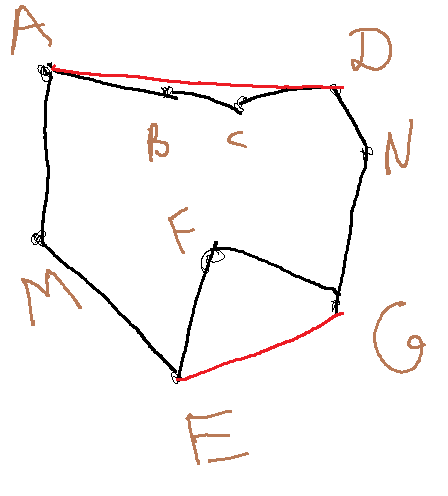
\includegraphics[scale=0.7]{1}\\
 	 в даном случае остается проверить для точки $U = (x, y), \; U \in ADGEM \cap U \notin FEG \cap U \notin ABCD$. \par
 	 Как же найти такие EFG? Как мы знаем уравнение прямой выглядит так: $\cfrac{x-x_1}{x_2 - x_1} = \cfrac{y-y_1}{y_2 -y_1}$. Теперь как определить что точка лежит справа? Можно просто посмоттеть где прямая через т U пересекает ось X например:\\
 	 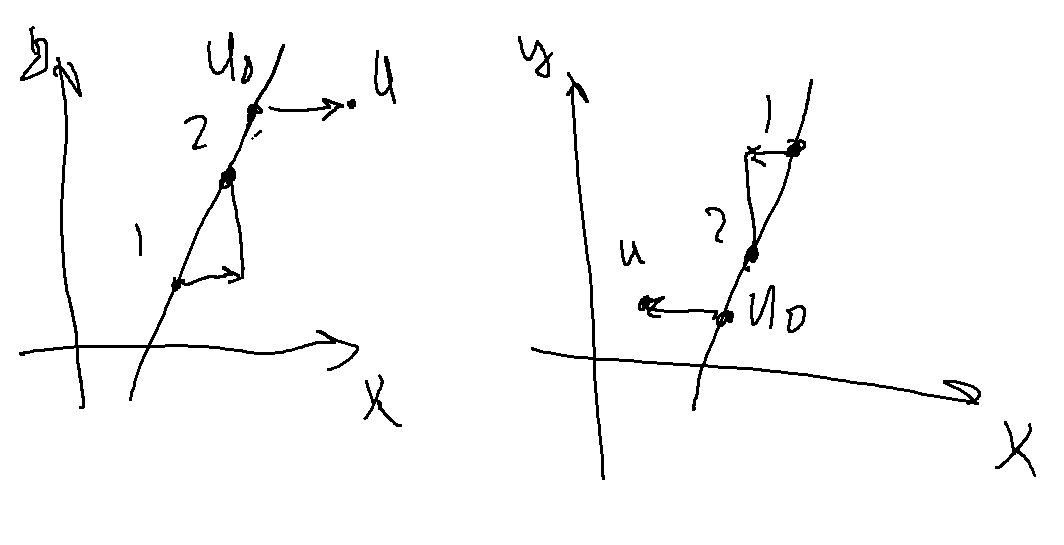
\includegraphics[scale=0.9]{2}\\
 	 \hspace*{1cm}Подставим y от U в уравнение получим:$x_3 =\cfrac{(y_U-y_1)(x_2 - x_1)}{y_2 -y_1} + x_1 $ тогда $U_0 = (x_3, y_U)$ тогда если $\cfrac{x_1 - x_2}{y_1 - y_2} > 0$ то U должна лежать правее точки $U_0$ получаем по знаку $x_U - \cfrac{(y_U-y_1)(x_2 - x_1)}{y_2 -y_1} - x_1\equiv x_2 - x_1$ иначе U должна лежать левее точки $U_0$ получаем по знак $x_U - \cfrac{(y_U-y_1)(x_2 - x_1)}{y_2 -y_1} - x_1\equiv -(x_2 - x_1)$ соеденяем получаем $x_U - \cfrac{(y_U-y_1)(x_2 - x_1)}{y_2 -y_1} - x_1\equiv \cfrac{x_1 - x_2}{y_1 - y_2}\cdot(x_2 - x_1)\implies (x_U -x_1) - \cfrac{(y_U-y_1)(x_2 - x_1)}{y_2 -y_1}\equiv \cfrac{(x_2 - x_1)^2}{y_2 - y_1}\implies(x_U -x_1)(y_2-y_1) - (y_U-y_1)(x_2 - x_1)\equiv (x_2 - x_1)^2 \implies(x_U -x_1)(y_2-y_1) - (y_U-y_1)(x_2 - x_1)\equiv1\implies(x_U -x_1)(y_2-y_1) > (y_U-y_1)(x_2 - x_1)$. Случай $U \in \cfrac{x-x_1}{x_2 - x_1} = \cfrac{y-y_1}{y_2 -y_1}$ нужно расмотреть отдельно но пусть в таком счучае будем считать, что принадлежит.\\ \\
 	 \hspace*{1cm}Итак формулы мы получили начнем писать код. Для начала хорошо бы создать класс точка с полями x, y. Так же прописать функцию поиска растояния и функции отрезка. Функцию отрезка можно получить вида $y=f(x)$ из ранее уже выведеной.
 	 \begin{verbatim}
 	 	import math
 	 	class point:
 	 	    def __init__(self, x:float, y:float):
 	 	        self.x = x
 	 	        self.y = y
 	 	
 	 	    def lenf(self, other):
 	 	        return math.sqrt((self.x - other.x)** 2 + (self.y - other.y)** 2)
 	 	
 	 	    def equatian(self, other, **printer):
 	 	        x_1, y_1 = self.x, self.y
 	 	        x_2, y_2 = other.x, other.y
 	 	        equatin = f"x * {(y_2 - y_1) / (x_2 - x_1)} - {x_1 * (y_2 - y_1) / (x_2 - x_1) + y_1}"
 	 	        if printer:
 	 	            print(f"y = {equatin}")
 	 	        return equatin
 	 	    
 	 	    def __eq__(self, other):
 	 	        return self.x == other.x and self.y == other.y
 	 	    
 	 	    def __hash__(self):
 	 	        return hash((self.x, self.y))
 	 \end{verbatim}
 	 И для красоты добавим функции print-а.
 	 \begin{verbatim}
 	 	    def __str__(self):
 	 	        return f"({self.x}, {self.y})"
 	 	    
 	 	    def __repr__(self):
 	 	        return f"<<{self.x}, {self.y}>>"
 	 \end{verbatim}
 	 \hspace*{1cm}Проверим "лежит точка справа от отрезка?": \\
 	 Функция принисает 3 точки 2 из которых задают направленую прямую и 3-я это проверяемая точка. Все необходимые функции мы уже вывели.
 	 \begin{verbatim}
 	 	def point_right_line(point1, point2, u) -> bool:
 	 	    return (u.x - point1.x) * (point2.y - point1.y
 	 	    ) > (u.y - point1.y) * (point2.x - point1.x)
 	 \end{verbatim}
 	 \hspace*{1cm}Проверяем лежит ли точка в выпуклой фигуре. 
 	 \begin{verbatim}
 	 def point_in_normal_figure(pl:List[Point], u:Point):
 	     if len(pl) < 3: print("errore!!!!! Beckend  line")
 	     orintation_right = point_right_line(pl[0], pl[1], pl[2])
 	     point1 = pl[0]
 	     for point2 in pl[1:]:
 	         if orintation_right != point_right_line(point1, point2, u):
 	             return False
 	         point1 = point2
 	     if orintation_right != point_right_line(pl[-1], plt[0], u):
 	         return False
 	     return True
 	 
 	
 	 \end{verbatim}
 	 
 	 \hspace*{1cm}А если многоугольник не выпуклый? Как уже было сказанно, будем делит на выпуклые фигуры и для них проверять лежит ли в них фигура. Самое сложное определить находится внутряняя часть фигуры справа или слева. Я предлагаю способ, который возможно будет работать не вегда, но в большинстве способов. Просто определить для каждого отрезка сколько точек лежит справа сколько слева. И так для всех и сложить. Получим два числа например r, l(r-спрва l-слева). И тогда если $r>l$ то спарава иначе слева. \par
 	 Тогда код будет выглядеть так:
 	 \begin{verbatim}
 	 def orintation_righ(main_fig:List[Point]):
 	     r, l = 0, 0
     	 temp_ln = len(main_fig)
 	     for i in range(temp_ln):
 	         for j in range(temp_ln):
 	             if j != i and j != (i + 1) % temp_ln:
 	                 if point_right_line(main_fig[i], main_fig[(i + 1) % temp_ln], main_fig[j]):
 	                 r += 1
 	             else:
 	                 l += 1
 	     return r > l
 	 
 	 
 	 
 	 def fig_decision(main_fig: List[Point]):
 	     main_fig = copy.copy(main_fig)
 	     added_fig = []
 	     orintation_right = orintation_righ(main_fig)
 	     count = 0
 	     i = 0
 	     while True:
 	         points = [main_fig[i % len(main_fig)], main_fig[(i + 2) %           len(main_fig)], main_fig[(i + 1) % len(main_fig)]]
 	         if (point_right_line(points[0], points[1], points[2]) and (not orintation_right)) or (
 	         (not point_right_line(points[0], points[1], points[2])) and orintation_right):
 	             count += 1
 	         else:
 	             added_fig += [points]
 	             main_fig.remove(main_fig[(i + 1) % len(main_fig)])
 	             count = 0
 	         i += 1
 	         if count == len(main_fig) + 3:
 	             break
 	     return (main_fig, added_fig)
 	 
 	 
 	 def point_in_bad_figure(main_fig: List[Point], added_fig: List[Point], u: Point):
 	     in_fig = point_in_normal_figure(main_fig, u)
 	     for i in added_fig:
 	         in_fig = in_fig and (not point_in_normal_figure(i, u))
 	     return in_fig
 	\end{verbatim}
 	\hspace*{1cm}И наконец функция разбиенияя на точки.
 	\begin{verbatim}
 	def bad_fig_to_point(main_fig:List[Point], step:float):
 	    fig_list = []
 	    maxx, maxy = minx, miny =  (
     	main_fig[0].x, main_fig[0].y)
 	    for i in main_fig:
 	        if i.x > maxx:
 	            maxx = i.x
 	        if i.x < minx:
 	            minx = i.x
 	        if i.y > maxy:
 	            maxy = i.y
 	        if i.y < miny:
 	            miny = i.y
 	    x_list = list(x * step for x in range(int(minx / step), int(maxx / step)))
 	    y_list = list(y * step for y in range(int(miny / step), int(maxy / step)))
 	    main_fig, added_fig = fig_decision(main_fig)
 	    for x, y in itertools.product(x_list, y_list):
 	        point = Point(x, y)
 	        if point_in_bad_figure(main_fig, added_fig, point):
 	            fig_list += [point]
 	    return fig_list
 	\end{verbatim}
 	\hspace*{1cm}Но есть еще один способ проверки принадлежности точки плоскости. Проведем через точку прямую, такую, что она будет пересекать грани фигуры(не вершины) тогда если пойти вдоль этой прямой от какого либо ее края, то каждое пересечение с гранью это вход или выход и тогда можно сказать, что если с каждой стороны от точки находится ничетное кол-во пересечений с гранями то мы получим что точка находится внутри фигуры. Теперь разберемся как получить прямую пересекающую только грани? Пусть у многоугольника к вершин тогда проведем к + 1 прямую и хотя бы одна не будет содержать вершин.\\
 	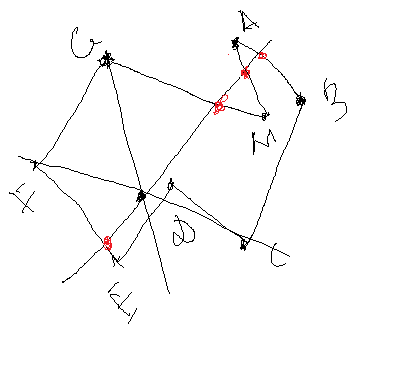
\includegraphics[scale=0.8]{3}\\
 	\hspace*{1cm}Итак начнем писать алгоритм класс точки возьмем из преведущего алгоритма. А метод проверки принадлежит ли точка прямой почти аналогичен функции проверки лежит ли точка справа от прямой, только знак неравенства нужно заметить равенством. Для класса Line нужно найти пересечение двух прямых. Для этого возьмем ур-е прямо\\\\
 	$\begin{cases}y = k_1 x + b_1\\   y = k_2 x + b_2\end{cases} \implies \begin{cases}(k_2 - k_1) x = b_1 - b_2\\   y = k_2 x + b_2\end{cases}\implies \begin{cases}x =\frac{ b_1 - b_2}{k_2 - k_1}\\   y = k_2 \frac{ b_1 - b_2}{k_2 - k_1} + b_2\end{cases}$
 	\begin{verbatim}
 	class Line:
 	    def __init__(self, p1:Point, p2:Point):
 	        self.p1 = p1
 	        self.p2 = p2
 	    
 	    def equatian(self):
 	        return list(map(float, 
 	        self.p1.equatian(self.p2).replace("x*", "").split("-")))
 	    
 	    def crossing(self, other):
 	        pr1 = self.p1.x == self.p2.x
 	        pr2 = other.p1.x == other.p2.x
 	        if pr1 and pr2:
 	            return None
 	        elif pr1:
 	            k2, b2 = other.equatian()
 	            return Point(self.p1.x, self.p1.x * k2 + b2)
 	        elif pr2:
 	            k1, b1 = self.equatian()
 	            return Point(other.p1.x, other.p1.x * k1 + b1)
 	        k1, b1 = self.equatian()
 	        k2, b2 = other.equatian()
 	        if k1 == k2:
 	            return None
 	        x = (b1 - b2) / (k2 - k1)
 	        y = k2 * x + b2
 	        return Point(x, y)
 	    
 	    def on(self, u:Point):
 	        return ((u.x - self.p1.x) * (self.p2.y - self.p1.y) == 
 	        (u.y - self.p1.y) * (self.p2.x - self.p1.x))
 	    
 	    def in(self, u:Point):
 	        x1, x2 = min(self.p1.x, self.p2.x), max(
 	        self.p1.x, self.p2.x)
 	        y1, y2 = min(self.p1.y, self.p2.y), max(
 	        self.p1.y, self.p2.y)
 	        return x1 <= u.x <= x2 and y1<= u.y <= y2
 	\end{verbatim}
 	\hspace*{1cm}Ок, а теперь сама функция. Мы получаем фигуру для нее нам понадобится список отрезков которыми она образованна и потом будем проводить прямую пока не найдем прямую которая не будет содержать вершину.
 	\begin{verbatim}
 	def point_in_fig(main_fig:List[Point], u:Point):
 	    if u in main_fig:return True
 	    lines = [Line(main_fig[i], main_fig[(i + 1) % len(main_fig)])
 	        for i in range(len(main_fig))]
 	    teastpoint = Point(u.x, u.y + 1)
 	    dx = 1
 	    while True:
 	        dx += 1
         	teastpoint.x += dx
         	teastpoint.y += 1
         	testline = Line(u, teastpoint)
         	if all(map(lambda x: not testline.on(x), main_fig)):
             	crossings = []
 	            for line in lines:
 	                c = testline.crossing(line)
 	                if c is not None:
 	                    if line.inl(c):
 	                        crossings += [c]
 	            if all(list(map(lambda x: x not in main_fig, crossings))):
                 	break
 	    cross = {"r": 0, "l": 0}
     	for c in crossings:
         	if c.y > u.y or (c.y == u.y and c.x > u.x):
             	cross["l"] += 1
         	else:
             	cross["r"] += 1
     
     	return cross["r"] % 2 == cross["l"] % 2 == 1
 	\end{verbatim}
 	\hspace*{1cm}Ок, а что на счет 3D? Думаю о направлении тут говорить нет смысла, так что прийдется использовать какой-то другой метод. Можно через каждую точку проводить прямую параллельную оси х и смотреть пересечения с фигурой если пересечения с каждой стороны нечетное кол-во то точка внутри иначе снаружи. Стоит учесть что это работает потому, что можно говорить о вхождении/выходе прямой из фигуры, но нужно сказать, что есть вид пересечение 2 граней в месте ребра и в таком месте может быть выход прямой из фигуры или его может и не быть. Эта проблема выпуклости, и решать ее будем так же, те разделем невыпуклую фигуру на выпуклые и обработаем включения/искючения.\\
 	\hspace*{1cm}Итак, начнем опять с точки.
 	\begin{verbatim}
 	class Point3:
 	    def __init__(self, x:float , y:float, z:float):
 	        self.x = x
 	        self.y = y
 	        self.z = z
 	\end{verbatim}
 	\hspace*{1cm}Теперь класс отрезка. Определять мы будем по 2 точкам. Так же добавим функцию проверки лежит ли точка на прямой. Алгоритм аналогичен 2D проверка истиности $\cfrac{x - x_1}{x_2 - x_1}$
 	\begin{verbatim}
 	class line:
 	    def __init__(self, p1:Point3, p2:Point3):
 	        self.p1 = p1
 	        self.p2 = p2
 	    
 	    def include(self, p:Point3):
 	        return round((self.p.y - self.p2.y) *
 	         (self.p1.x - self.p2.x) - (self.p.x - self.p2.x)
 	          * (self.p1.y - self.p2.y), 5) == round(
 	          (self.p2.y - self.p.y) *  (self.p1.z - self.p2.z) - 
 	          (self.p2.z - self.p.z)
 	          * (self.p1.y - self.p2.y), 5) == 0
 	       
    \end{verbatim}
    \hspace*{1cm}Теперь плоскость. Ур-е плоскости $Ax + By + Cz = 1$. Для определения плоскости достаточно трех точек. Решим ур-е:\\$\begin{cases}
    Ax_1 + By_1 + Cz_1 = 1 \\ Ax_2 + By_2 + Cz_2 = 1 \\ Ax_3 + By_3 + Cz_3 = 1
    \end{cases}$\\$\begin{cases}
    A = 1 - B\frac{y_1}{x_1} - C\frac{z_1}{x_1} \\  B = 1 - A\frac{x_2}{y_2} - C\frac{z_2}{y_2}  \\ C = 1 - B\frac{y_3}{z_3} - A\frac{x_3}{z_3}
    \end{cases}$\\$\begin{cases}
    A = 1 - B\frac{y_1}{x_1} - C\frac{z_1}{x_1} \\  B = 1 - A\frac{x_2}{y_2} - \left(1 - B\frac{y_3}{z_3} - A\frac{x_3}{z_3}\right)\frac{z_2}{y_2}  \\ C = 1 - B\frac{y_3}{z_3} - A\frac{x_3}{z_3}
    \end{cases}$\\ $\begin{cases}
    A = 1 - B\frac{y_1}{x_1} - C\frac{z_1}{x_1} \\  B(1 + \frac{y_3}{z_3}\frac{z_2}{y_2}) = 1  - \frac{z_2}{y_2}  - A(\frac{x_3}{z_3}\frac{z_2}{y_2} + \frac{x_2}{y_2})  \\ C = 1 - B\frac{y_3}{z_3} - A\frac{x_3}{z_3}
    \end{cases}$\\$\begin{cases}
    A = 1 - B\frac{y_1}{x_1} - C\frac{z_1}{x_1} \\  B = \cfrac{1  - \frac{z_2}{y_2}  - A(\frac{x_3}{z_3}\frac{z_2}{y_2} + \frac{x_2}{y_2})}{(1 + \frac{y_3}{z_3}\frac{z_2}{y_2})}  \\ C = 1 - B\frac{y_3}{z_3} - A\frac{x_3}{z_3}
    \end{cases}$\\$\begin{cases}
    A = 1 - B\frac{y_1}{x_1} - C\frac{z_1}{x_1} \\  B =  \cfrac{1  - \frac{z_2}{y_2}  - A(\frac{x_3z_2 + x_2z_3}{z_3y_2} )}{(\frac{z_3y_2 + y_3z_2}{z_3y_2})}  \\ C = 1 - \left( \cfrac{1  - \frac{z_2}{y_2}  - A(\frac{x_3z_2 + x_2z_3}{z_3y_2} )}{(\frac{z_3y_2 + y_3z_2}{z_3y_2})}\right) \frac{y_3}{z_3} - A\frac{x_3}{z_3}
    \end{cases}$\\$\begin{cases}
    A = 1 - B\frac{y_1}{x_1} - C\frac{z_1}{x_1} \\  B =  \cfrac{z_3y_2  - z_2z_3  - A(x_3z_2 + x_2z_3 )}{(z_3y_2 + y_3z_2)}  \\ C = 1 -  \cfrac{y_3y_2  - z_2y_3  - A(\frac{y_3x_3z_2}{z_3} + x_2y_3 )}{(z_3y_2 + y_3z_2)} - A\frac{x_3}{z_3}
    \end{cases}$\\$\begin{cases}
    A = 1 - B\frac{y_1}{x_1} - C\frac{z_1}{x_1} \\  B =  \cfrac{z_3y_2  - z_2z_3}{(z_3y_2 + y_3z_2)} - A\cfrac{(x_3z_2 + x_2z_3 )}{(z_3y_2 + y_3z_2)}  \\ C = 1 -  \cfrac{y_3y_2  - z_2y_3}{(z_3y_2 + y_3z_2)} - A\left(\cfrac{(\frac{y_3x_3z_2}{z_3} + x_2y_3)}{(z_3y_2 + y_3z_2)} + \frac{x_3}{z_3}\right)
    \end{cases}$\\$\begin{cases}
    A = 1 - B\frac{y_1}{x_1} - C\frac{z_1}{x_1} \\  B =  \cfrac{z_3y_2  - z_2z_3}{(z_3y_2 + y_3z_2)} - A\cfrac{(x_3z_2 + x_2z_3 )}{(z_3y_2 + y_3z_2)}  \\ C = 1 -  \cfrac{y_3y_2  - z_2y_3}{(z_3y_2 + y_3z_2)} - A\left(\cfrac{2y_3x_3z_2 + x_2y_3z_3 + z_3y_2x_3 }{(z_3y_2 + y_3z_2)z_3}\right)
    \end{cases}$\\$
    A= \cfrac{1 - \left(\cfrac{z_3y_2  - z_2z_3}{(z_3y_2 + y_3z_2)} \right)\frac{y_1}{x_1}  - \left( 1 -  \cfrac{y_3y_2  - z_2y_3}{(z_3y_2 + y_3z_2)}\right)\frac{z_1}{x_1}}{\left(1 + \cfrac{(x_3z_2 + x_2z_3 )}{(z_3y_2 + y_3z_2)}\frac{y_1}{x_1} + \cfrac{2y_3x_3z_2 + x_2y_3z_3 + z_3y_2x_3 }{(z_3y_2 + y_3z_2)}\frac{z_1}{z_3x_1}\right) } $\\$
    A= \cfrac{(z_3y_2 + y_3z_2)x_1z_3 - \left((z_3y_2  - z_2z_3) \right)z_3y_1  - \left( (z_3y_2 + y_3z_2) -  (y_3y_2  - z_2y_3)\right)z_3z_1}{\left((z_3y_2 + y_3z_2)z_3 + (x_3z_2 + x_2z_3 )z_3y_1 + (2y_3x_3z_2 + x_2y_3z_3^2 + y_2x_3z_3)z_1\right) } $\\$  B =  \cfrac{z_3y_2  - z_2z_3}{(z_3y_2 + y_3z_2)} - A\cfrac{(x_3z_2 + x_2z_3 )}{(z_3y_2 + y_3z_2)} $ \\$ C =  1 - B\frac{y_3}{z_3} - A\frac{x_3}{z_3}$\\
    Та форма ур-я плоскости почти верна, но есть один граничный случай, когда она не работает, тогда на помощь приходит:\\$\begin{cases}
    Ax_1 + By_1 + Cz_1 = 0 \\ Ax_2 + By_2 + Cz_2 = 0 \\ Ax_3 + By_3 + Cz_3 = 0
    \end{cases}$\\$\begin{cases}
    A = 0 - B\frac{y_1}{x_1} - C\frac{z_1}{x_1} \\  B = 0 - A\frac{x_2}{y_2} - C\frac{z_2}{y_2}  \\ C = 0 - B\frac{y_3}{z_3} - A\frac{x_3}{z_3}
    \end{cases}$\\$\begin{cases}
    A = 0 - B\frac{y_1}{x_1} - C\frac{z_1}{x_1} \\  B = 0 - A\frac{x_2}{y_2} - C\frac{z_2}{y_2}  \\ C = A\frac{x_2}{y_2}\frac{y_3}{z_3} + C\frac{z_2}{y_2}\frac{y_3}{z_3} - A\frac{x_3}{z_3}
    \end{cases}$\\$\begin{cases}
    A = 0 - B\frac{y_1}{x_1} - C\frac{z_1}{x_1} \\  B = 0 - A\frac{x_2}{y_2} - C\frac{z_2}{y_2}  \\ C =\cfrac{ A(\frac{x_2}{y_2}\frac{y_3}{z_3} - \frac{x_3}{z_3})}{1 - \frac{z_2}{y_2}\frac{y_3}{z_3}}
    \end{cases}$\\$\begin{cases}
    A = 0 - B\frac{y_1}{x_1} - C\frac{z_1}{x_1} \\  B = 0 - A\frac{x_2}{y_2} - \cfrac{ A(\frac{x_2}{y_2}y_3 - x_3)}{z_3y_2 - z_2y_3}z_2  \\ C =\cfrac{ A(\frac{x_2}{y_2}y_3 - x_3)}{z_3 - \frac{z_2}{y_2}y_3}
    \end{cases}$\\$\begin{cases}
    A = 0 - B\frac{y_1}{x_1} - C\frac{z_1}{x_1} \\  B = 0 - A\left(\frac{x_2}{y_2} - \cfrac{ (\frac{x_2}{y_2}y_3 - x_3)}{z_3y_2 - z_2y_3}z_2\right)  \\ C =A\left(\cfrac{ (\frac{x_2}{y_2}y_3 - x_3)}{z_3 - \frac{z_2}{y_2}y_3}\right)
    \end{cases}$\\$\begin{cases}
    A = 0 + A\left(\frac{x_2}{y_2} - \cfrac{ (\frac{x_2}{y_2}y_3 - x_3)}{z_3y_2 - z_2y_3}z_2\right)\frac{y_1}{x_1} - A\left(\cfrac{ (\frac{x_2}{y_2}y_3 - x_3)}{z_3 - \frac{z_2}{y_2}y_3}\right)\frac{z_1}{x_1} \\  B = 0 - A\left(\frac{x_2}{y_2} - \cfrac{ (\frac{x_2}{y_2}y_3 - x_3)}{z_3y_2 - z_2y_3}z_2\right)  \\ C =A\left(\cfrac{ (\frac{x_2}{y_2}y_3 - x_3)}{z_3 - \frac{z_2}{y_2}y_3}\right)
    \end{cases}$
    \\
    Для того что-бы определить лежит точка на плоскости достаточно подставить координаты точки в ур-е плоскости. А вот что-бы определить лежит ли точка на гране прийдется писать ту же функцию которую мы уже писали но в 3D, но мы схитрим. Точка лежит внутри фигуры если\\ \hspace*{2cm} 1. она лежит в той же плоскости \\  \hspace*{2cm} 2. Если она лежитв проекции фигуры.\\ Тогда для удобства будем проецтровать грань на плоскость образованнную осями o.X, o.Y. Учтем что при проецировании плоскость не должна быть паралельна o.Z, и если такое случится будем проецирвать на o.Z, o.Y или на o.X, o.Z.\\
    \hspace*{1cm} А теперь найдем пересечение прямой и плоскости. Для этого опять решим систему: \\ $ \begin{cases}Ax + By + Cz = 1 \\ \cfrac{x-x_1}{x_2 - x_1} = \cfrac{y-y_1}{y_2 - y_1} \\ \cfrac{z-z_1}{z_2 - z_1} = \cfrac{y-y_1}{y_2 - y_1}  \end{cases}$\\
    $ \begin{cases}x = 1 - \cfrac{B}{A}y - \cfrac{C}{A}z  \\  y = \cfrac{(y_2 - y_1)(x-x_1)}{x_2 - x_1} + y_1 \\ z = \cfrac{(z_2 - z_1)(y-y_1)}{y_2 - y_1} + z_1  \end{cases}$\\
    $ \begin{cases}x = 1 - \cfrac{B}{A}y - \cfrac{C}{A}z  \\  y = \cfrac{(y_2 - y_1)(x-x_1)}{x_2 - x_1} + y_1 \\ z = \cfrac{(y_2 - y_1)(x-x_1)}{x_2 - x_1}\cfrac{(z_2 - z_1)}{y_2 - y_1} + z_1  \end{cases}$\\
     $ \begin{cases}x = 1 - \cfrac{B}{A}y - \cfrac{C}{A}z  \\  y = \cfrac{(y_2 - y_1)(x-x_1)}{x_2 - x_1} + y_1 \\ z = \cfrac{(z_2 - z_1)(x-x_1)}{x_2 - x_1} + z_1  \end{cases}$\\
     $ \begin{cases}x = 1 - \cfrac{B}{A}\left(\cfrac{(y_2 - y_1)(x-x_1)}{x_2 - x_1} + y_1\right) - \cfrac{C}{A}\left(\cfrac{(z_2 - z_1)(x-x_1)}{x_2 - x_1} + z_1\right)  \\  y = \cfrac{(y_2 - y_1)(x-x_1)}{x_2 - x_1} + y_1 \\ z =  \cfrac{(z_2 - z_1)(x-x_1)}{x_2 - x_1} + z_1 \end{cases}$ \\
     $ x  = \cfrac{A - B\left(y_1 - \cfrac{(y_2 - y_1)x_1}{x_2 - x_1}\right) - C\left(z_1-\cfrac{(z_2 - z_1)x_1}{x_2 - x_1} \right) }{A  + B\cfrac{(y_2 - y_1)}{x_2 - x_1} + C\cfrac{(z_2 - z_1)}{x_2 - x_1}} \\  y = \cfrac{(y_2 - y_1)(x-x_1)}{x_2 - x_1} + y_1 \\ z =  \cfrac{(z_2 - z_1)(x-x_1)}{x_2 - x_1} + z_1 $ \\
     \hspace*{-1cm}$ x  = \cfrac{A(x_2 - x_1) - B\left(y_1(x_2 - x_1) - (y_2 - y_1)x_1\right) - C(z_1(x_2 - x_1) -(z_2 - z_1)x_1) }{A(x_2 - x_1)  + B(y_2 - y_1) + C(z_2 - z_1)} \\  y = \cfrac{(y_2 - y_1)(x-x_1)}{x_2 - x_1} + y_1 \\ z =  \cfrac{(z_2 - z_1)(x-x_1)}{x_2 - x_1} + z_1 $ \\
     Если x1 = x2 получим \\$ \begin{cases} By = 1 - Ax_1 - Cz \\  z = \cfrac{(z_2 - z_1)(y-y_1)}{y_2 - y_1} + z_1  \end{cases}$\\$ \begin{cases} y = \cfrac{ 1 - Ax_1 + C\cfrac{(z_2 - z_1)y_1}{y_2 - y_1} - Cz_1}{B + C\cfrac{(z_2 - z_1)}{y_2 - y_1}} \\  z = \cfrac{(z_2 - z_1)(y-y_1)}{y_2 - y_1} + z_1  \end{cases}$ \\$ \begin{cases} y = \cfrac{ (y_2 - y_1) - Ax_1(y_2 - y_1) + C(z_2 - z_1)y_1 - Cz_1(y_2 - y_1)}{B(y_2 - y_1) + C(z_2 - z_1)} \\  z = \cfrac{(z_2 - z_1)(y-y_1)}{y_2 - y_1} + z_1  \end{cases}$
    \\
    Осталось это перенести в код:
    \begin{verbatim}
    class plane:
        def __init__(self, lines:List[Points]):
            
    \end{verbatim}
    
    \hspace*{-2cm}$ \overrightarrow{C} = \left(\begin{bmatrix}
    y1 z1\\ y2 z2
    \end{bmatrix},-\begin{bmatrix}
    x1 z1\\ x2 z2
    \end{bmatrix},\begin{bmatrix}
    x1 y1\\ x2 y2
    \end{bmatrix}\right)= \left(y1z2 - z1y2, x2z1 - x1z2, x1y2 - x2y1\right)$\\
    $ \cfrac{x - x_1}{x_2 - x_1} = \cfrac{y - y_1}{y_2 - y_1} = \cfrac{z - z_1}{z_2 - z_1} = \lambda \implies \begin{cases}
    x = \lambda (x_2 - x_1) + x_1\\
    y = \lambda (y_2 - y_1) + y_1\\
    z = \lambda (z_2 - z_1) + z_1
    \end{cases}$\\ \newpage
	\hspace{-1cm}$\begin{cases}
	x = \lambda (x_2 - x_1) + x_1\\
	y = \lambda (y_2 - y_1) + y_1\\
	z = \lambda (z_2 - z_1) + z_1\\
	Ax + By + Cz + D = 0
	\end{cases}$\\
	$\begin{cases}
	x = \lambda (x_2 - x_1) + x_1\\
	y = \lambda (y_2 - y_1) + y_1\\
	z = \lambda (z_2 - z_1) + z_1\\
	\lambda = \cfrac{-Ax_1 - By_1 - Cz_1 - D}{A(x_2 - x_1) + B(y_2 - y_1) + C(z_2 - z_1)}
	\end{cases}$
 \end{document}